\PID \mnImportant
Испитати асимптотску стабилност система који су дефинисани датом диференцном једначином у операторском облику
\begin{multicols}{2}
    \begin{enumerate}[label=(\alph*)]
    \item $ \left(\EE + \dfrac14 \right)^2\left(\EE - \dfrac12 \right)y[n] = x[n]$;
    \item $(\EE^2 - \EE \sqrt2 + 1) y[n] = x[n]$;
    \item $(\EE^2 + 1)^2 y[n] = x[n]$;
    \item $\left(\EE - \dfrac12 \right)(\EE - 2) y[n] = x[n]$.
    \end{enumerate}
\end{multicols} \noindent

\RESENJE 
%
\begin{figure}[b!]
    \centering
    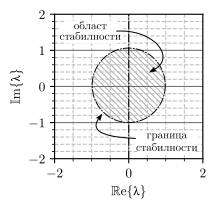
\includegraphics{fig/stab_edit.pdf}
    \caption{Уз стабилност дискретних система.}
    \label{fig:\ID.stab}
\end{figure}
%
Појам асимтотске стабилности код дискретних система потпуно је еквивалентан оном како је дефинисан 
за континуалне системе, односно како је описано у задатку \refz{ct_stab}. На сличан начин, 
У табели \ref{tab:\ID.1} приказано је понашање карактеристичних функција (к.ф.) које потичу од коренова карактеристичног 
полинома (к.п.) код дискретних система 
%
У табели се препознају сличности али и значајне разлике код утицаја коренова карактеристичног полинома 
на стабилност система. Област стабилности у комплексној равни јесте отворени јединични круг $|\uplambda| < 1$, 
а граница стабилности је јединична кружница $|\uplambda| = 1$, као што је илустровано на слици
\ref{fig:\ID.stab}. На тај начин, критеријум стабилности се 
може исказати на исти начин као за континуалне системе, односно: 
систем је асимптотски стабилан уколико има корене који се налазе искључиво у области стабилности; 
маргинално је стабилан уколико има једноструке корене на граници стабилности, а асимптотски је нестабилан 
уколико има корене потпуно ван области стабилности.
%
\noindent
\begin{table}[ht!]
    \centering
\begin{tabular}{l|l}
    \begin{minipage}{0.3\textwidth}
    \textbf{Корен к. п.}
    \end{minipage} & \textbf{Понашање к. ф.} \\ 
    %
    \begin{minipage}{0.3\textwidth}
    $\uplambda \in \mathbb R$, једноструки корен
    \end{minipage}
    &
    \begin{minipage}{0.6\textwidth}
    $\uplambda^{n} \begin{cases}
        \to 0, & \text{ако је $|\uplambda| < 1$} \\
        = 1, & \text{ако је $\uplambda = 1$} \\    
        \to \infty, & \text{ако је $|\uplambda| > 1$} \\    
    \end{cases}$
    \end{minipage}\\[7mm]
    %
    \begin{minipage}{0.3\textwidth}
    $\uplambda \in \mathbb R$, $k$-тоструки корен
    \end{minipage}
    &
    \begin{minipage}{0.6\textwidth}
        $\uplambda^{n}, \ldots, n^{k-1} \uplambda^{n}
        \begin{cases}
            \to 0 ,&  \text{ако је $\uplambda < |1|$} \\
            \to \infty ,&  \text{ако је $\uplambda \geq 1$} \\
        \end{cases}$
    \end{minipage}\\[7mm]
    %
    \begin{minipage}{0.3\textwidth}
    $\uplambda = \uprho \ee^{\jj\Omega} \in \mathbb C$, једноструки \\ корен
    \end{minipage}
    &
    \begin{minipage}{0.6\textwidth}
    $\uprho^n \sin(\Omega n), \uprho^n \cos(\Omega n)
    \begin{cases}
        \to 0 ,&  \text{ако је $\uprho < 0$} \\
        \text{осцилаторно} ,&  \text{ако је $\uprho = 0$} \\
        \to \infty ,&  \text{ако је $\uprho > 0$} \\
    \end{cases}$
    \end{minipage} \\[7mm]
    %
    \begin{minipage}{0.3\textwidth}
    $\uplambda = \uprho \ee^{\jj\Omega} \in \mathbb C$, $k$-тоструки \\ корен
    \end{minipage}
    &
    \begin{minipage}{0.6\textwidth}
    $
    \begin{matrix}
        \uprho^n \sin(\Omega n), \uprho^n \cos(\Omega n) \\
        \vdots \\ 
        \uprho^n n^{k-1} \sin(\Omega n), \uprho^n n^{k-1} \cos(\Omega n)
    \end{matrix}
    \begin{cases}
        \to 0 ,&  \text{ако је $\uprho < 1$} \\
        \to \infty ,&  \text{ако је $\uprho \geq 1$} 
    \end{cases}$
    \end{minipage} \\
\end{tabular}
\caption{Асимптотско понашање карактеристичних функција, преглед.}
\label{tab:\ID.1}
\end{table}

(a) Корени карактеристичниг полинома су $\uplambda_1 = -\dfrac14$ (двоструки) и $\uplambda_2 = \dfrac12$. 
Пошто се оба корена налазе у области стабилности, дати систем је асимптотски стабилан. 

(б) Корени карактеристичног полинома су $\uplambda_{12} = \ee^{\pm \jj\uppi/4}$. Пошто постоји једноструки пар 
комплексно конјугованих коренова на граници стабилности систем је гранично стабилан. 

(в) Корени карактреристичног полиома су $\uplambda_{12} = \pm\jj$ (двоструки пар). Пошто постоје двоструки корени 
на граници стабилности, дати систем је асимптотски нестабилан.

(г) Корени карактеристичног полинома су $\uplambda_1 = \dfrac12$, и $\uplambda_2=2$. Пошто постоји барем један 
корен потпуно ван области стабилности, систем је асимптотски нестабилан. 

